%%%%%%%%%%%%%%%%%%%%%%%%%%%%%%%%%%%%%%%%%
% University/School Laboratory Report
% LaTeX Template
% Version 3.1 (25/3/14)
%
% This template has been downloaded from:
% http://www.LaTeXTemplates.com
%
% Original author:
% Linux and Unix Users Group at Virginia Tech Wiki 
% (https://vtluug.org/wiki/Example_LaTeX_chem_lab_report)
%
% License:
% CC BY-NC-SA 3.0 (http://creativecommons.org/licenses/by-nc-sa/3.0/)
%
%%%%%%%%%%%%%%%%%%%%%%%%%%%%%%%%%%%%%%%%%

%----------------------------------------------------------------------------------------
%	PACKAGES AND DOCUMENT CONFIGURATIONS
%----------------------------------------------------------------------------------------

\documentclass{article}
\usepackage[version=3]{mhchem} % Package for chemical equation typesetting
\usepackage{siunitx} % Provides the \SI{}{} and \si{} command for typesetting SI units
\usepackage[final]{graphicx}
\usepackage{natbib} % Required to change bibliography style to APA
\usepackage{amsmath} % Required for some math elements 
\usepackage{pythonhighlight}
\usepackage{commath}
\usepackage{listings}
\usepackage{xcolor}
\usepackage{gensymb}
\usepackage{subcaption}
\captionsetup[figure]{font=small,labelfont=small}
\usepackage{float}
\usepackage[margin=1in]{geometry}

\lstset { %
	language=C++,
	backgroundcolor=\color{black!5}, % set backgroundcolor
	basicstyle=\footnotesize,% basic font setting
}
\setlength\parindent{0pt} % Removes all indentation from paragraphs
\usepackage{hyperref}

\renewcommand{\labelenumi}{\alph{enumi}.} % Make numbering in the enumerate environment by letter rather than number (e.g. section 6)

%\usepackage{times} % Uncomment to use the Times New Roman font

%----------------------------------------------------------------------------------------
%	DOCUMENT INFORMATION
%----------------------------------------------------------------------------------------

\title{Implementation of a Raytracer \\ in C++ \\ Computer Graphics Project (Rendering Track)} % Title

\author{Alhajras Algdairy \\alhajras.algdairy@gmail.com, 4963555, aa382} % Author name

\date{\today} % Date for the report

\begin{document}

\maketitle % Insert the title, author and date

\begin{center}
\begin{tabular}{l r}
University: & University of Freiburg \\ % Date the experiment was performed
Instructor: &Dr.-Ing. Matthias Teschner % Instructor/supervisor
\end{tabular}
\end{center}
\clearpage
% If you wish to include an abstract, uncomment the lines below
% \begin{abstract}
% Abstract text
% \end{abstract}

%----------------------------------------------------------------------------------------
%	SECTION 1
%----------------------------------------------------------------------------------------
\tableofcontents
\clearpage
\section{Objective}

The aim of this report is to document the steps which are important to implement a basic Raytracer in C++ language.  As a beginner myself into the Computer graphics world, I will be explaining the tools, concept, equations, algorithms and sources that have been used during this small project.  


% If you have more than one objective, uncomment the below:
%\begin{description}
%\item[First Objective] \hfill \\
%Objective 1 text
%\item[Second Objective] \hfill \\
%Objective 2 text
%\end{description}

\subsection{Milestones}
\label{definitions}
\begin{itemize}
	\item Create PPM file and show an image, this includes understanding how images are generated.
	\item Show a sphere because it is a trivial object.
	\item Show a Triangle and implement an object array so it can be used in the future for rendering more than one object.
	\item Show a cube and a complex object by using the triangle array or mesh renderer.
	\item Create a benchmark tests in order to compare the basic functionality of the raytracer and after adding more features to it in the future.
	\item Add transformations: Translation, Rotation, Scaling, Reflection
	and Shearing.
	\item Phong model, and benchmark tests.
	\item Transparency and reflection
\end{itemize}

 \clearpage
%----------------------------------------------------------------------------------------
%	SECTION 2
%----------------------------------------------------------------------------------------

\section{Creating an image}
\subsection{Concept}
There are so many formats, ppm file, PPM stands for Portable Pixmap Format, which was developed in the 1980s to allow image files to be transferred between different computer platforms.

\begin{figure}[H]
	
	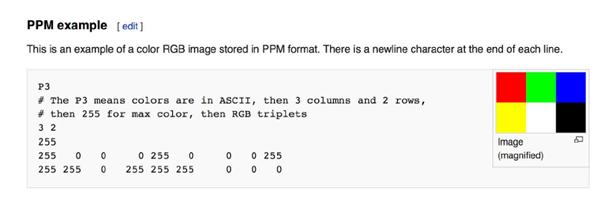
\includegraphics[width=250pt]{C:/D/University/Semester_4/Raytracer/lab_report_1/assignment_2/images/1.png}
	
	\caption{PPM format example.}
	\label{fig:boat1}
\end{figure}


\subsection{Results}

\begin{figure}[H]
	\begin{center}
		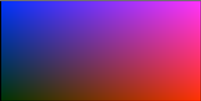
\includegraphics[width=250pt]{C:/D/University/Semester_4/Raytracer/lab_report_1/assignment_2/images/2.png}
		
		\caption{Hello world image in PPM format}
		\label{fig:boat1}
	\end{center}
\end{figure}
 \clearpage

%----------------------------------------------------------------------------------------
%	SECTION 3
%----------------------------------------------------------------------------------------
\section{Rays}
\subsection{Concept}
Optical ray tracing describes a method for producing visual images constructed in 3D computer graphics environments, with more photorealism than either ray casting or scanline rendering techniques. It works by tracing a path from an imaginary eye through each pixel in a virtual screen, and calculating the color of the object visible through it.
All raytracers are using something called rays. Let’s think of a ray as a function \[p (t) = A + tB\] Here p is a 3D position along a line
in 3D. A is the ray origin and B is the ray direction.

\begin{figure}[H]
	
	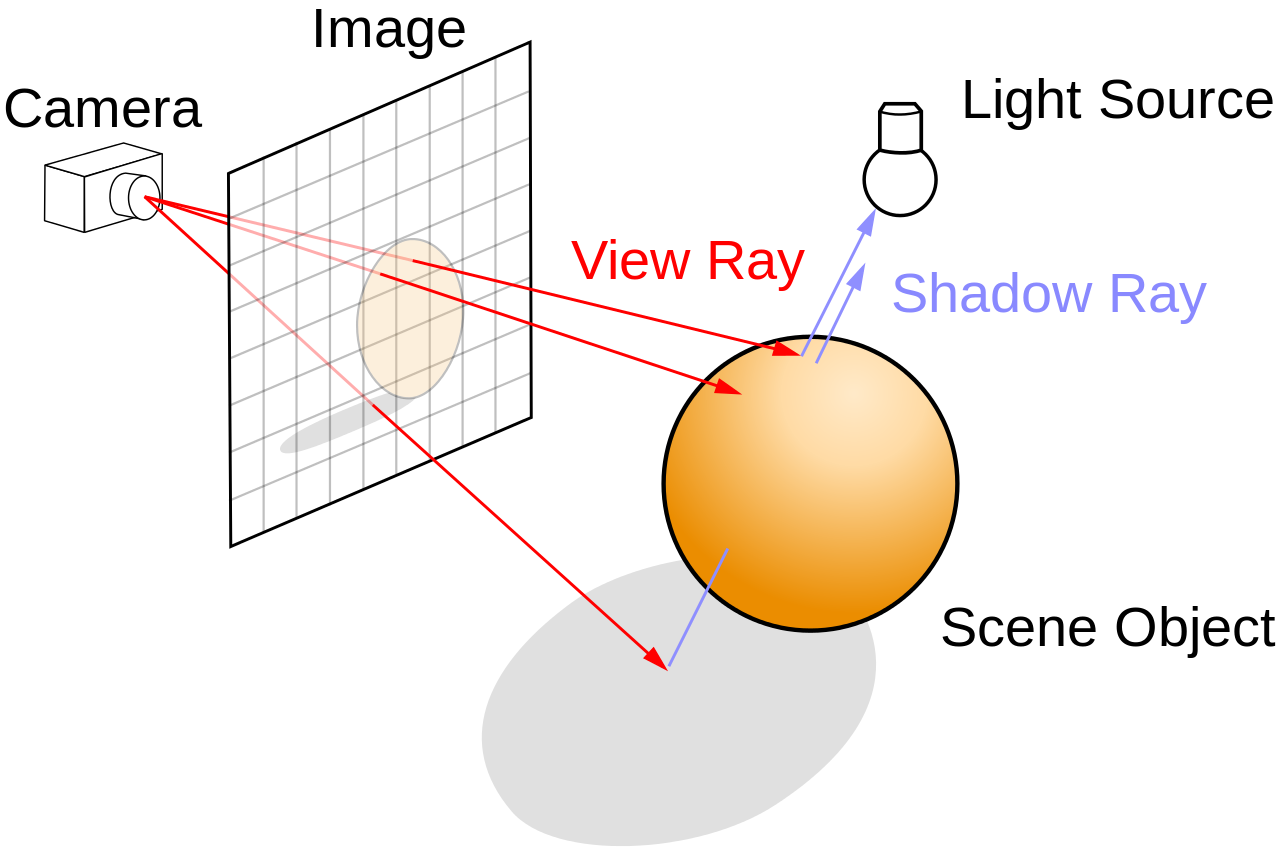
\includegraphics[width=250pt]{C:/D/University/Semester_4/Raytracer/lab_report_1/assignment_2/images/3.png}
	
	\caption{The ray-tracing algorithm builds an image by extending rays into a scene and bouncing them off surfaces and towards sources of light to approximate the color value of pixels. \href{https://en.wikipedia.org/wiki/Ray_tracing_(graphics)}{LaTeX-Tutorial}.}
	\label{fig:boat1}
\end{figure}

\subsection{Pseudo code}
\begin{lstlisting}
#ifndef RAY_H
#define RAY_H

#include "vec3.h"


class ray {
	public:
	ray() {}
	ray(const point3& origin, const vec3& direction)
	: orig(origin), dir(direction), tm(0)
	{}
	
	ray(const point3& origin, const vec3& direction, double time)
	: orig(origin), dir(direction), tm(time)
	{}
	
	point3 origin() const  { return orig; }
	vec3 direction() const { return dir; }
	double time() const    { return tm; }
	
	point3 at(double t) const {
		return orig + t*dir;
	}
	
	public:
	point3 orig;
	vec3 dir;
	double tm;
};

#endif
\end{lstlisting}

\subsection{Results}
\begin{figure}[H]
	
	
\includegraphics[width=250pt]{C:/D/University/Semester_4/Raytracer/lab_report_1/assignment_2/images/4.png}
	
	\caption{Output of the blank background without an object by using rays}
	\label{fig:boat1}
\end{figure}

\section{Adding a sphere}
\subsection{Concept}
People often use spheres in ray tracers because
calculating whether a ray hits a sphere is pretty straightforward.

The general equation of a sphere is: \[ \abs{(x - c)^2} = r^2\] 
Subsituting ray formula in spher we get: 
\[ (A + tB - c)^2.(A + tB - c)^2 = r^2\] 

The form of a quadratic formula is now observable. (This quadratic equation is an instance of Joachimsthal's equation.[2])

By solving the equation we get three different cases as shown in figure below.
\begin{figure}[H]
	
	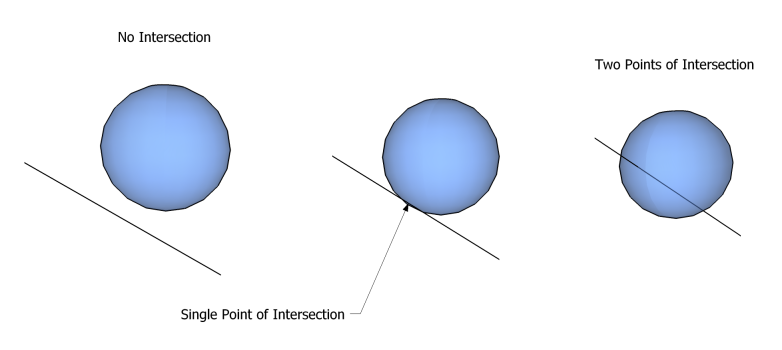
\includegraphics[width=250pt]{C:/D/University/Semester_4/Raytracer/lab_report_1/assignment_2/images/5.png}
	
	\caption{The three possible line-sphere intersections:
		1. No intersection.
		2. Point intersection.
		3. Two point intersection.}
	\label{fig:boat1}
\end{figure}
\href{https://en.wikipedia.org/wiki/Line%E2%80%93sphere_intersection}{LaTeX-Tutorial}.
\subsection{Pseudo code}
\begin{lstlisting}
bool hit_sphere(const vec3& center, float radius, const ray& r) {
	vec3 oc = r.origin() - center;
	float a = dot(r.direction(), r.direction());
	float b = 2.0 * dot(oc, r.direction());
	float c = dot(oc, oc) - radius * radius;
	float discrimnant = b * b - 4 * a * c;
	return (discrimnant > 0);
}
\end{lstlisting}


\subsection{Results}
\begin{figure}[H]
		\begin{center}
	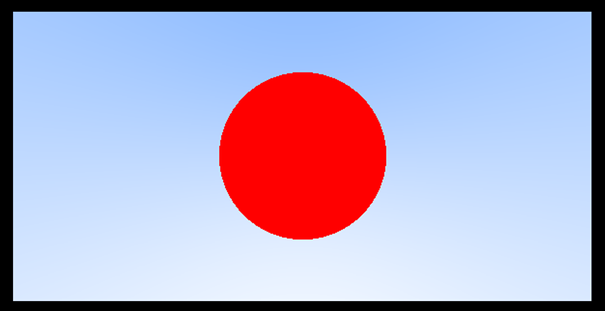
\includegraphics[width=250pt]{C:/D/University/Semester_4/Raytracer/lab_report_1/assignment_2/images/6.png}
	
	\caption{Rendering a simple Sphere}
	\label{fig:boat1}
		\end{center}
\end{figure}



\section{Adding a Triangle}
\subsection{Concept}
Computing the intersection of a ray with a primitive such as a sphere, is not difficult. However, since it is difficult to model most 3D objects with spheres alone, it is necessary to use some other types of primitive to represent more complex objects (objects of arbitrary shape).
Instead of working with complex primitives such as NURBS or Bezier patches, we can convert every object into a triangle mesh and compute the intersection of a ray with every triangle in this mesh. 
By solving the equation we get three different cases as shown in figure below.
\begin{figure}[H]
	
	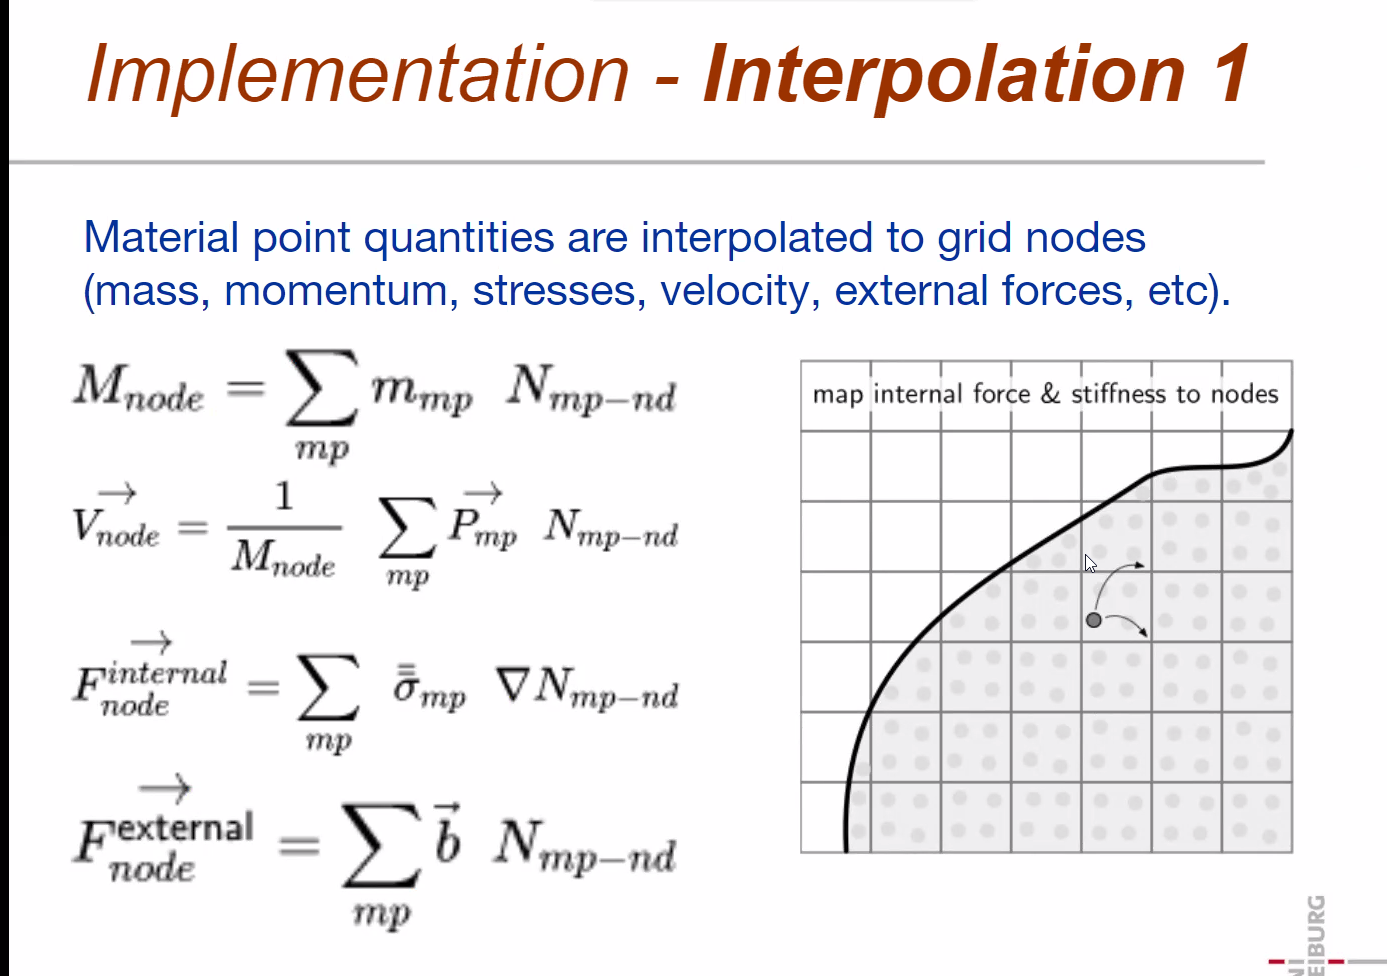
\includegraphics[width=250pt]{C:/D/University/Semester_4/Raytracer/lab_report_1/assignment_2/images/8.png}
	\label{fig:boat1}
\end{figure}
\href{https://en.wikipedia.org/wiki/Line%E2%80%93sphere_intersection}{LaTeX-Tutorial}
	
		\begin{figure}[H]
		\begin{center}
			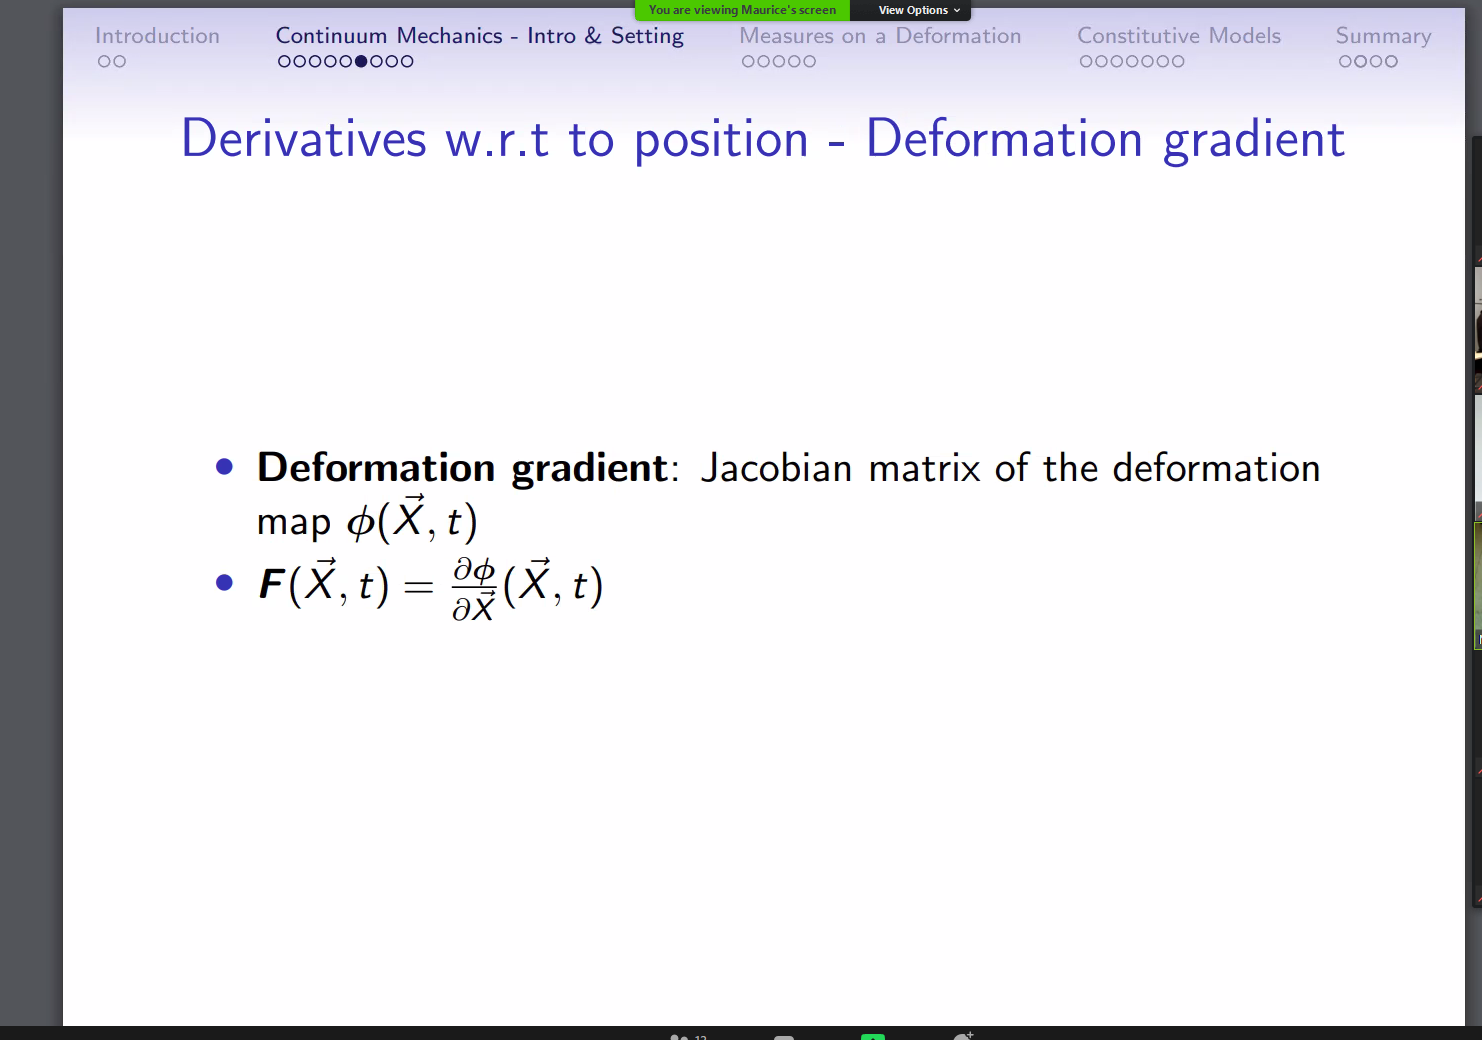
\includegraphics[width=250pt]{C:/D/University/Semester_4/Raytracer/lab_report_1/assignment_2/images/9.png}
			
			\caption{Rendering a simple Sphere}
			\label{fig:boat1}
		\end{center}
	\end{figure}
	\subsection{Pseudo code}
	\begin{lstlisting}
Vec3f edge0 = v1 - v0; 
Vec3f edge1 = v2 - v1; 
Vec3f edge2 = v0 - v2; 
Vec3f C0 = P - v0; 
Vec3f C1 = P - v1; 
Vec3f C2 = P - v2; 
if (dotProduct(N, crossProduct(edge0, C0)) > 0 && 
dotProduct(N, crossProduct(edge1, C1)) > 0 && 
dotProduct(N, crossProduct(edge2, C2)) > 0) return true; // P is inside the triangle 
		}
	\end{lstlisting}
	
	
	\subsection{Results}
	\begin{figure}[H]
		\begin{center}
			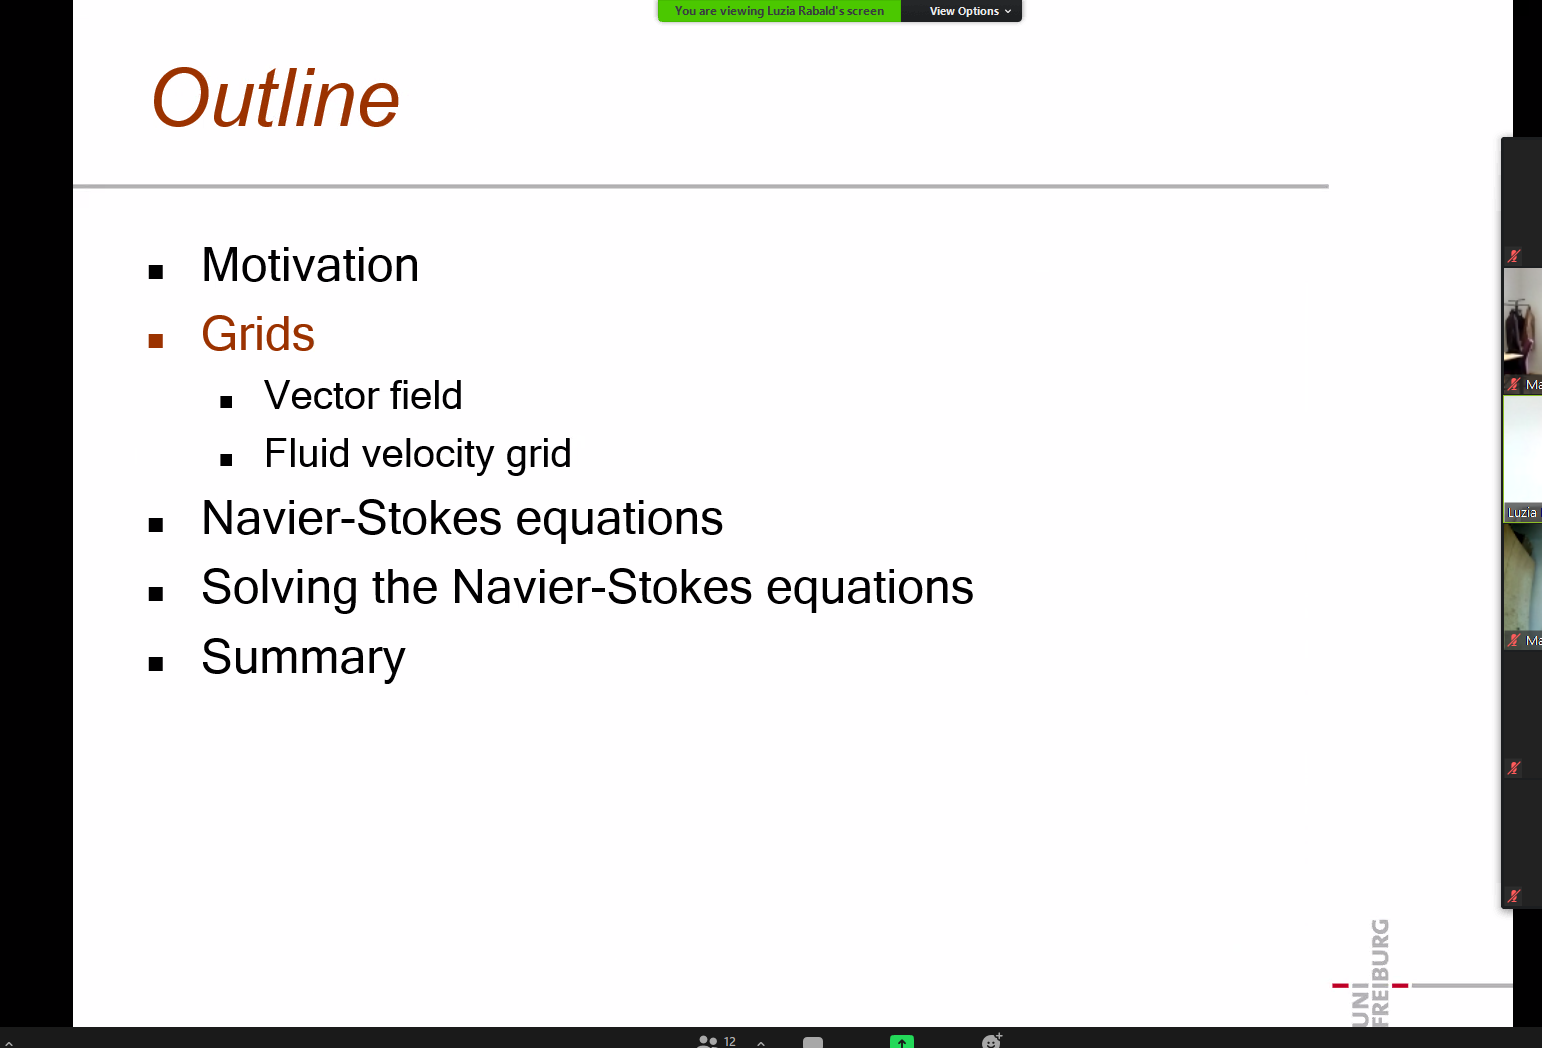
\includegraphics[width=250pt]{C:/D/University/Semester_4/Raytracer/lab_report_1/assignment_2/images/7.png}
			
			\caption{Rendering a simple Triangle}
			\label{fig:boat1}
		\end{center}
	\end{figure}

\clearpage


\section{Shading}
\subsection{Concept}

Rendering a scene needs two steps the first step is solving the visibility issue, this means which object is visible to the camera and what its shape, second step is Shading, this deals with the color of the object and its intensity. Shading include also how objects color affect each other, for example having light hits the object will make its color look brighter, on the other hand regions which light doesn't hit or reach will have dark color or shadow. In this chapter shading concepts will be discussed and implemented.  The main key to shading is calculating the amount of light that hits a point lets call it P. 

The computed light at a point P depends on the following: 

\begin{itemize}
	\item Light illuminated by source source  $L^{source}$  in real life usually lamp, fire or the sun, it can have any color and intensity but here we will use white color. 
	\item Surface illumination $L^{surface}$.
	\item Light reflected from the surface $L^{reflected}$.
	\item The observation angle / looking at angle / camera. 
\end{itemize}




\subsubsection{Lambert’s Cosine Law}
Lambert's cosine law says that the amount of light energy arriving at a surface is proportional to the cosine of the angle between the light direction and the surface normal. Illumination strength at a surface is proportional to the cosine of the angle between $l$ and $n$, the angel will be denoted as $\theta$, the next three cases illustrate the relationship between the  $L^{source}$ and  $L^{surface}$:

The  $L^{surface}$,$ L^{source}$ relation is: $L^{surface} = L^{source}.\cos \theta $
\begin{itemize}
	\item $L^{surface} = L^{source}$, if $\theta = 0\degree$.
	\item $L^{surface} = 0$, if $\theta = 90\degree$.
    \item $0 < L^{surface} < L^{source}$, if $0\degree < \theta  < 90\degree$.
\end{itemize}

\subsubsection{Phong reflection model }
Phong reflection is an empirical model of local illumination. It describes the way a surface reflects light as a combination of the diffuse reflection of rough surfaces with the specular reflection of shiny surfaces. It is based on Phong's informal observation that shiny surfaces have small intense specular highlights, while dull surfaces have large highlights that fall off more gradually. The model also includes an ambient term to account for the small amount of light that is scattered about the entire scene.
\\


\begin{figure}[ht]
	\begin{subfigure}{.3\textwidth}
		\centering
		% include first image
		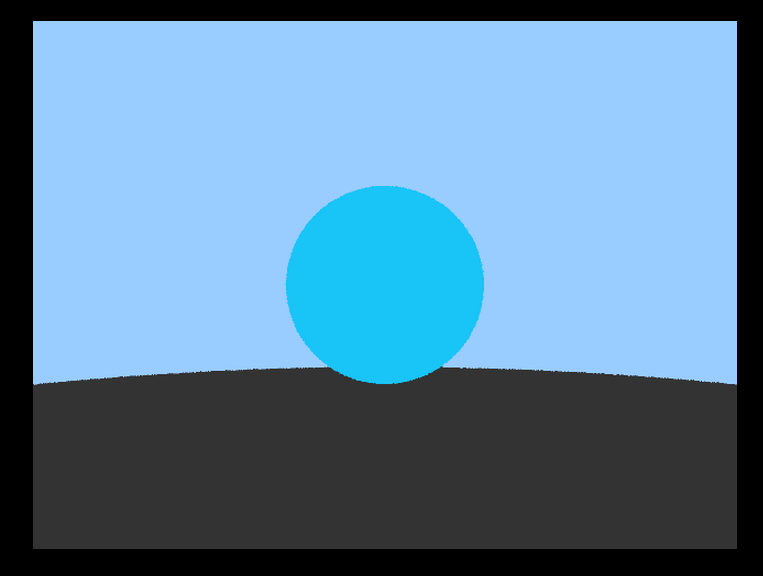
\includegraphics[width=.8\linewidth]{C:/D/University/Semester_4/Raytracer/lab_report_1/assignment_2/images/amb_reflection.png}  
		\caption{}
		\label{fig:sub-first}
	\end{subfigure}
	\begin{subfigure}{.3\textwidth}
		\centering
		% include second image
		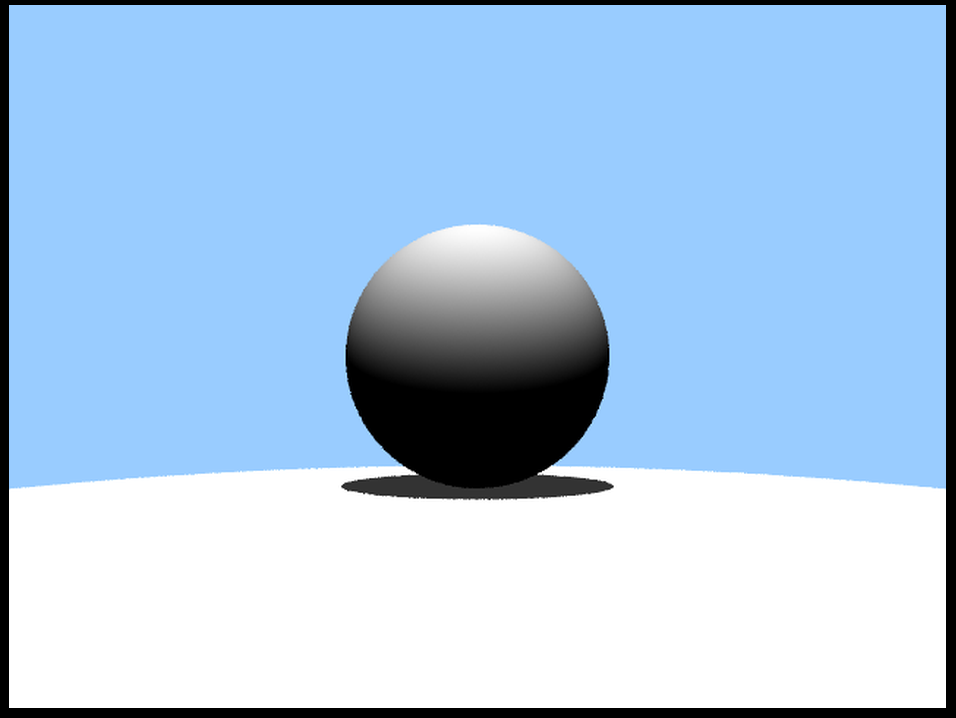
\includegraphics[width=.8\linewidth]{C:/D/University/Semester_4/Raytracer/lab_report_1/assignment_2/images/diff_reflection_2.png}  
		\caption{}
		\label{fig:sub-second}
	\end{subfigure}
	\begin{subfigure}{.3\textwidth}
		\centering
		% include second image
		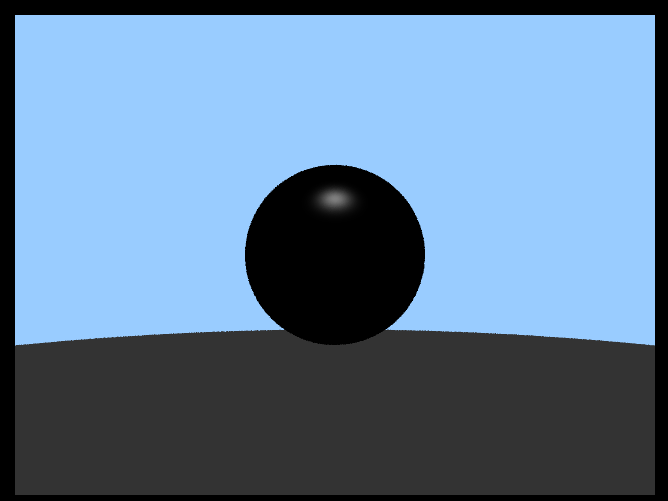
\includegraphics[width=.8\linewidth]{C:/D/University/Semester_4/Raytracer/lab_report_1/assignment_2/images/spec_reflection_2.png}  
		\caption{}
		\label{fig:sub-third}
	\end{subfigure}
	
	\caption{(a). Ambient .(b). Diffuse. (c). Specular (Glossy)}
	\label{fig:fig}
\end{figure}


\begin{itemize}
	\item \textbf{Ambient reflection}
		\begin{equation}
L^{amb} = \rho \otimes L^{indirect}
		\end{equation}
	
	\begin{itemize}
		\item $\rho$, is the surface color
		\item $L^{indirect}$ , is the light reflected from other surfaces and objects, excluded the direct light ($L^{source}$)
	\end{itemize}
	\item \textbf{Diffuse reflection} 

					\begin{equation}
L^{diff} =  L^{source}.(n.l) \otimes \rho 
			\end{equation}
				\begin{itemize}
		\item $L^{source}$, is the light source color and intensity which usually white. 
		\item $n$ and $l$ , are the representation of the Lambert's cosine law, where n is the normal surface vector  and l is the indecent light coming from the light source.
	\end{itemize}
	\item \textbf{Specular reflection} 

								\begin{equation}
L^{spec} =  L^{source}.(n.l).(r.v)^m \otimes \rho^{white} 
			\end{equation}
				\begin{itemize}
		\item $r$, which is the direction that a perfectly reflected ray of light would take from this point on the surface. 
		\item $v$, which is the direction pointing towards the viewer (such as a virtual camera).
		\item $m$, which is a shininess constant for this material, which is larger for surfaces that are smoother and more mirror-like. When this constant is large the specular highlight is small.
	\end{itemize}
\end{itemize}

The overall illumination on the surface can be computed by summing up the three components that make up \textit{Phong model}:

\begin{equation}
	L^{surface}= L^{amb} + \sum_{n=1}^{lights} (L_n^{diff} + L_n^{spec})
\end{equation}



\begin{figure}[ht]
	\begin{subfigure}{.3\textwidth}
		\centering
		% include first image
		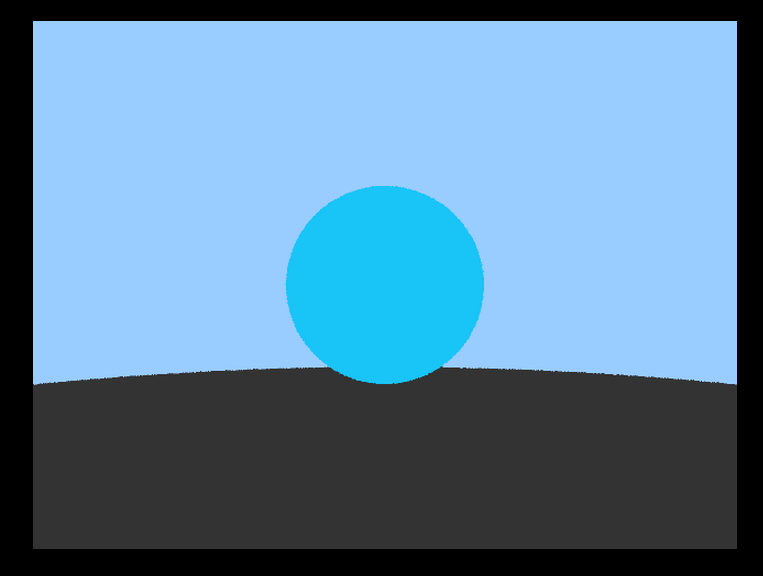
\includegraphics[width=.8\linewidth]{C:/D/University/Semester_4/Raytracer/lab_report_1/assignment_2/images/amb_reflection.png}  
		\caption{}
		\label{fig:sub-first}
	\end{subfigure}
	\begin{subfigure}{.3\textwidth}
		\centering
		% include second image
		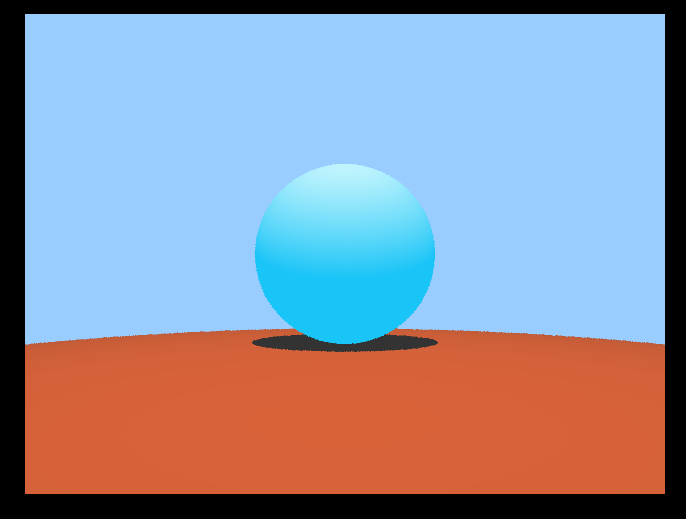
\includegraphics[width=.8\linewidth]{C:/D/University/Semester_4/Raytracer/lab_report_1/assignment_2/images/diff_reflection.png}  
		\caption{}
		\label{fig:sub-second}
	\end{subfigure}
	\begin{subfigure}{.3\textwidth}
		\centering
		% include second image
		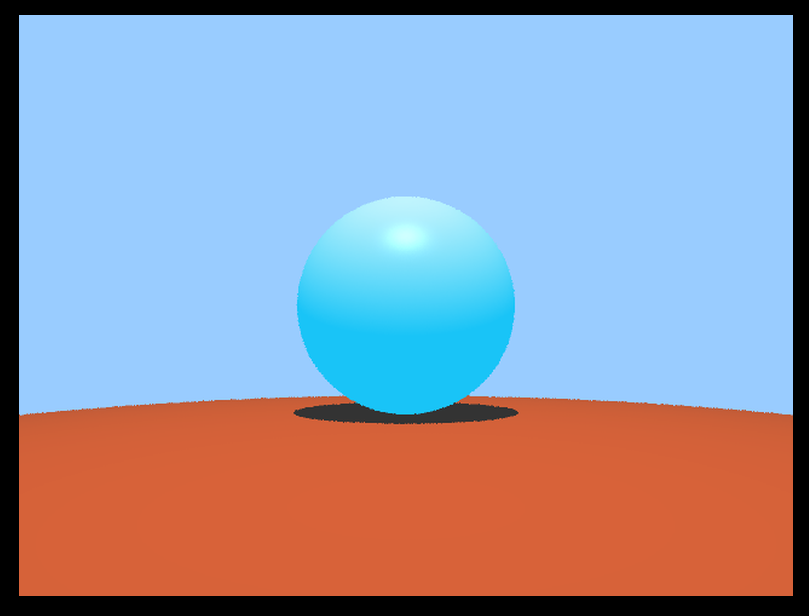
\includegraphics[width=.8\linewidth]{C:/D/University/Semester_4/Raytracer/lab_report_1/assignment_2/images/spec_reflection.png}  
		\caption{}
		\label{fig:sub-third}
	\end{subfigure}
	
			\begin{subfigure}{.3\textwidth}
		\centering
		% include second image
		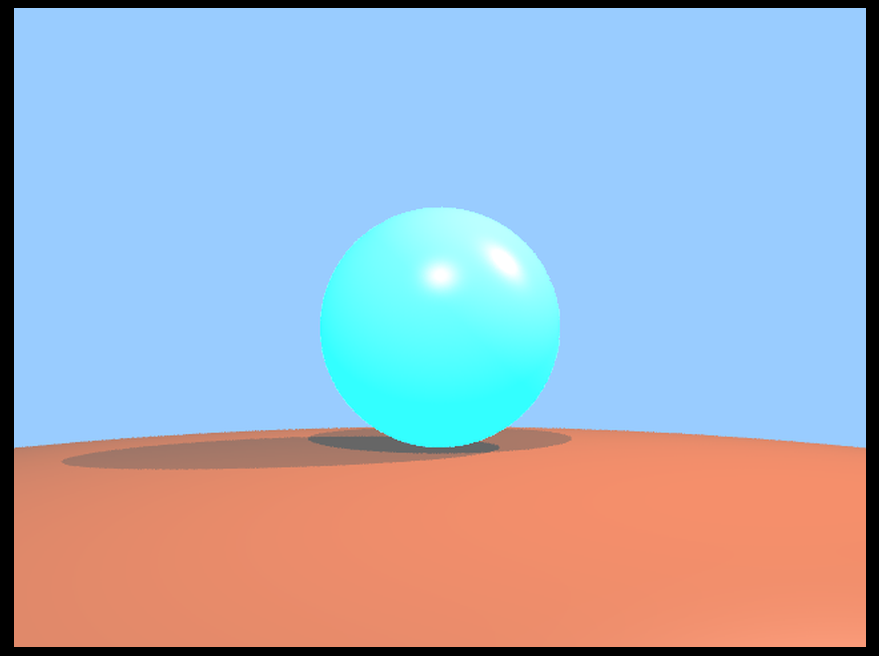
\includegraphics[width=.8\linewidth]{C:/D/University/Semester_4/Raytracer/lab_report_1/assignment_2/images/multi_shadow_multi_spec.png}  
		\caption{}
		\label{fig:sub-third}
	\end{subfigure}
	\caption{(a). Ambient .(b). Diffuse + Ambient. (c). Diffuse + Ambient + Specular (Glossy). (d). Multiable lights that generates brighter surface and multiple shadows.}
	\label{fig:fig}
\end{figure}


\section{Materials}
	      \subsection{Concept}
	      In raytracing one of the important topics is to give the object a material type, this can be: Glossy, Diffuse, Transparent and Subsurface
	      scattering, each material has different surface reflection and refraction properties, some surfaces reflect the light equally such as diffuse surfaces, some are reflecting light into a dominant direction as Glossy surfaces, some material such as water will reflect some light but also refract some.
	      \\ 
	      In the previous chapter we discussed diffuse and specular (Glossy) surfaces, in this chapter we will implement a refraction surface because it has an interesting properties. 
	      
	      \subsection{Refraction}
	      Refraction phenomenon happens when the light pass from one medium to a different medium.
	      Figure 12 illustrates this phenomenon, $I$ is the incident light ray, $R$ is the reflected light where $N$ is the normal vector to the surface which is water (in blue), the reflected angle  $\theta2$ is equal to the incident angle $\theta1$, in addition to the reflected light there is a refracted light $T$, the direction of $T$ depends on the $\theta1$ and \textit{refractive index, $\eta$} ( Describes how fast light travels through the material).
	      
	      Refraction is described by the \textit{Snell's law}, which states that for a given pair of media, the ratio of the sines of the angle of incidence $\theta1$ and angle of refraction $\theta2$ is equivalent to the opposite ratio of the indices of refraction: 
	      
	      \begin{equation}
\frac{sin(\theta_1)}{sin(\theta_2)} = \frac{\eta_2}{\eta_1} 
	      \end{equation}
      
	      
	\begin{figure}[H]
	\begin{center}
		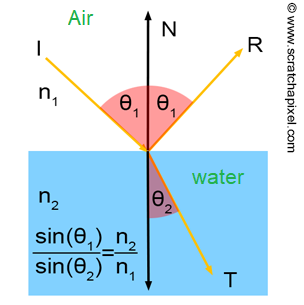
\includegraphics[width=150pt,height=150pt]{C:/D/University/Semester_4/Raytracer/lab_report_1/assignment_2/images/refraction.png}
		
		\caption{Incident light $I$ in the air hitting water surface, $R$ is reflected light and $T$ is the transmitted and refracted light, $n$ is \textit{refractive index, $\eta$  } Resource: \href{https://www.scratchapixel.com/images/upload/shading-intro/shad-refraction6.png?}{scratchapixel.com}.
			]}
	\end{center}
\end{figure}

\subsection{Fresnel}
The amount of reflected vs. refracted light can be computed using what we call the \textit{Fresnel equations}, where $F_R$ is reflected light portion and $F_T$ is the portion transmitted through the material. 

\begin{equation}
 F_R = \dfrac{1}{2}(\left( \dfrac{\eta_2 \cos\theta_1 - \eta_1 \cos \theta_2}{\eta_2 \cos\theta_1 + \eta_1 \cos \theta_2} \right)^2 + \left( \dfrac{\eta_1 \cos\theta_2 - \eta_2 \cos \theta_1}{\eta_1 \cos\theta_2 + \eta_2 \cos \theta_1} \right)^2)
\end{equation}



\begin{equation}
F_T= 1 - F_R 
\end{equation}


\subsection{Results}
Figure 13 shows the refraction phenomenon where the settings had a red glossy sphere passing behind a transparent sphere with an refractive index, $\eta$ not equal to the air we are assuming it is any kind of liqued with big $\eta$ that it refract the light with a big angle. As it can be noticed the red sphere looks larger than it should be and also inverted, moreover the ground is inverted as well, 
\begin{figure}[H]
	\begin{subfigure}{.3\textwidth}
		\centering
		% include first image
		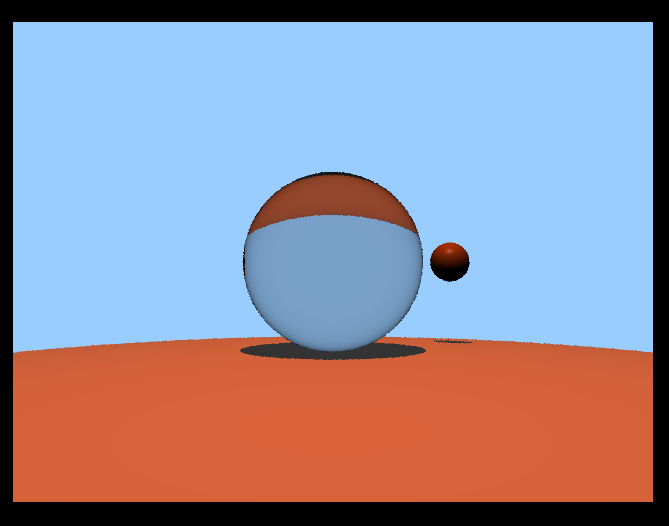
\includegraphics[width=.8\linewidth]{C:/D/University/Semester_4/Raytracer/lab_report_1/assignment_2/images/refraction_3.png}  
		\caption{}
		\label{fig:sub-first}
	\end{subfigure}
	\begin{subfigure}{.3\textwidth}
		\centering
		% include second image
		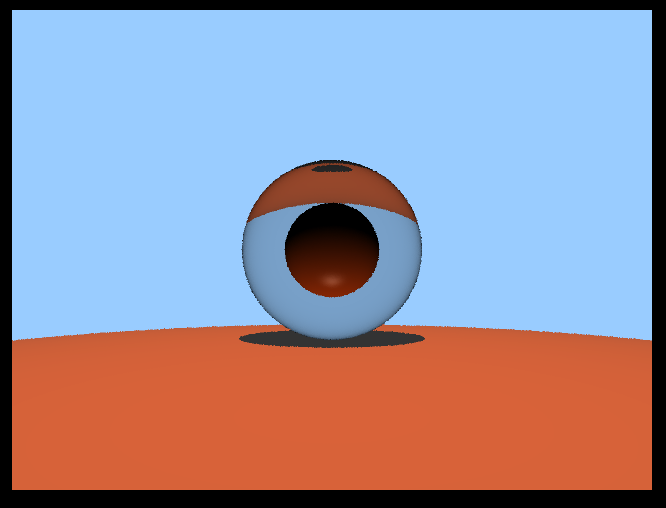
\includegraphics[width=.8\linewidth]{C:/D/University/Semester_4/Raytracer/lab_report_1/assignment_2/images/refraction_0.png}  
		\caption{}
		\label{fig:sub-second}
	\end{subfigure}
	\begin{subfigure}{.3\textwidth}
	\centering
	% include second image
	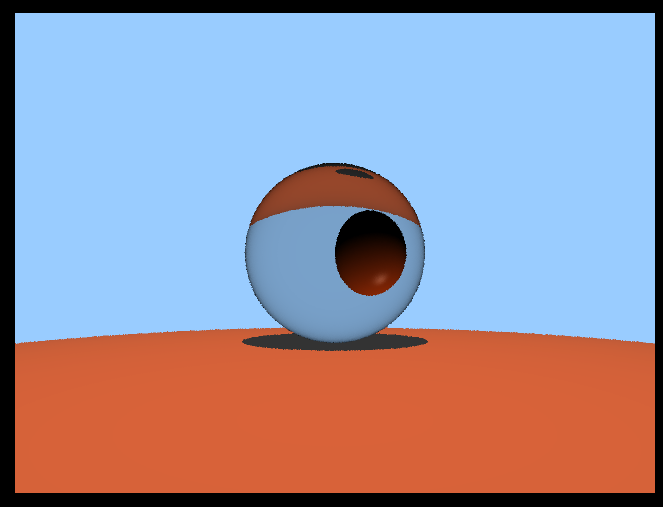
\includegraphics[width=.8\linewidth]{C:/D/University/Semester_4/Raytracer/lab_report_1/assignment_2/images/refraction__0_5.png}  
	\caption{}
	\label{fig:sub-third}
\end{subfigure}

	\caption{(a). Glass sphere refract the ground inverted upside down. (b). Glass sphere refract the ground and red sphere directly behind it inverted. (c). Glass sphere refract the ground and red sphere behind it inverted with an angle}
	\label{fig:fig}
\end{figure}
\clearpage

\section{Texture}
In computer graphics, the application of a type of surface to a 3D image. A texture can be uniform, such as a brick wall, or irregular, such as wood grain or marble. The common method is to create a 2D bitmapped image of the texture, called a "texture map," which is then "wrapped around" the 3D object. An alternate method is to compute the texture entirely via mathematics instead of bitmaps. Textures are so useful, they  reduce the geometric complexity of a scene by mapping a bit directly to an image or having a mathematical equation that can easily represent the surface color, they also reduce the number of vertices, and it reduces the modeling and rendering time. 

We will only consider some mathematical patterns and not image mapping, procedural texturing
define how to use the texture value, e.g. replace the original surface color with the texture color
linearly combine the original surface color with the texture
multiply, add, subtract surface color and texture color.


\begin{figure}[ht]
	\begin{subfigure}{.3\textwidth}
		\centering
		% include first image
		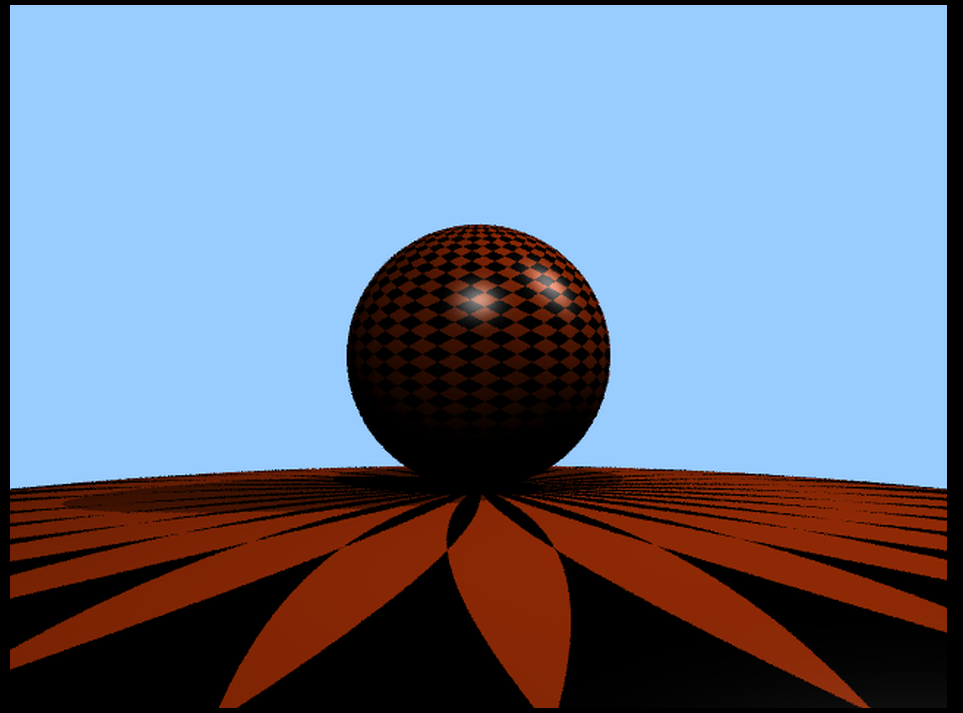
\includegraphics[width=.8\linewidth]{C:/D/University/Semester_4/Raytracer/lab_report_1/assignment_2/images/texture_1.png}  
		\caption{}
		\label{fig:sub-first}
	\end{subfigure}
	\begin{subfigure}{.3\textwidth}
		\centering
		% include second image
		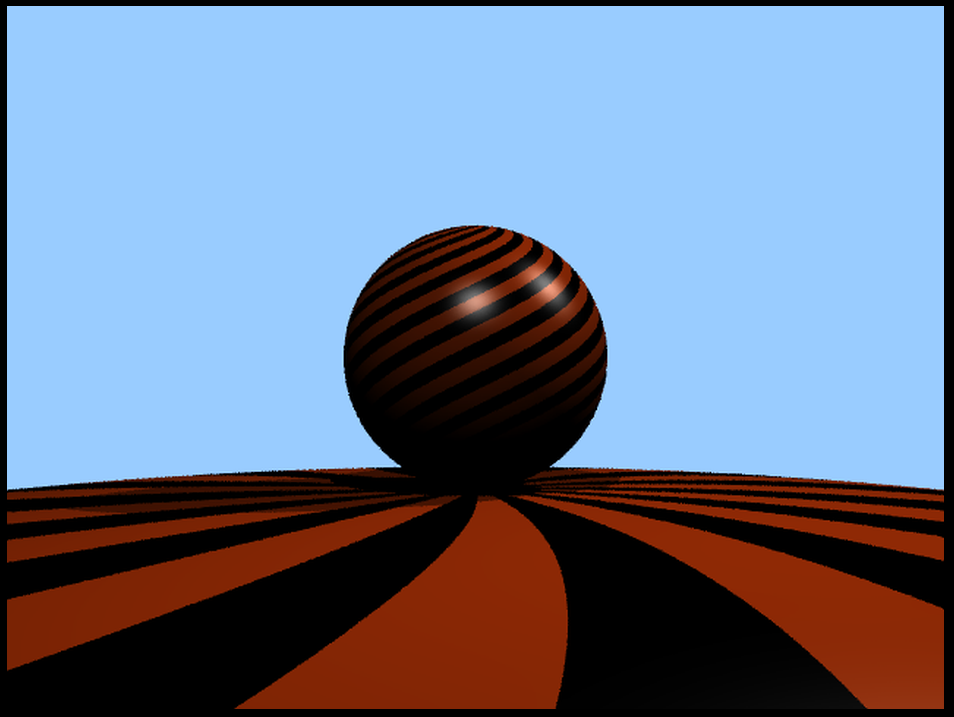
\includegraphics[width=.8\linewidth]{C:/D/University/Semester_4/Raytracer/lab_report_1/assignment_2/images/texture_2.png}  
		\caption{}
		\label{fig:sub-second}
	\end{subfigure}
	\begin{subfigure}{.3\textwidth}
		\centering
		% include second image
		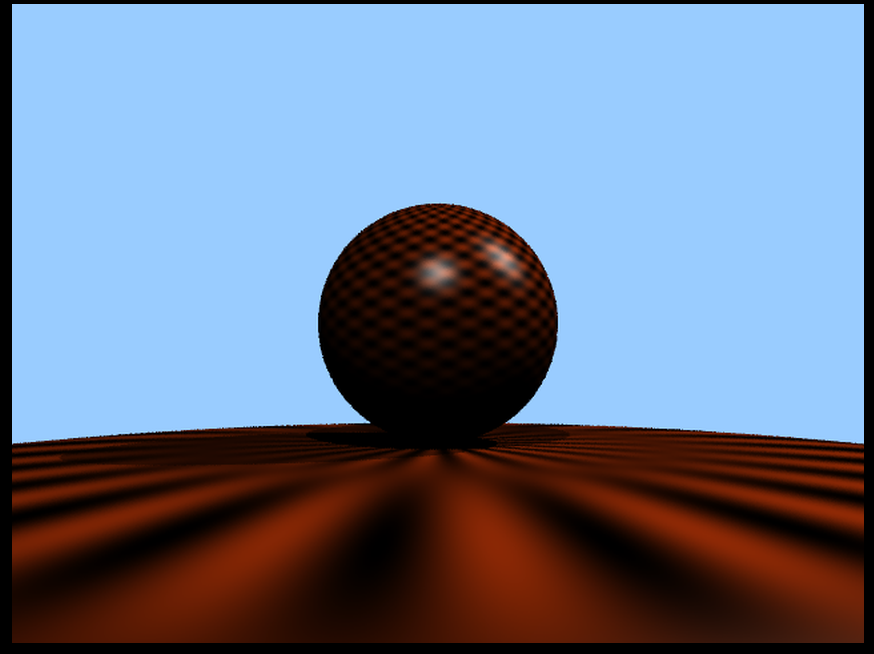
\includegraphics[width=.8\linewidth]{C:/D/University/Semester_4/Raytracer/lab_report_1/assignment_2/images/texture_3.png}  
		\caption{}
		\label{fig:sub-third}
	\end{subfigure}
	
	\caption{(a), (b) and (c) show different pattern for textures that can be generated by mathematical equations to map x and y value to different color value.}
	\label{fig:fig}
\end{figure}


\subsection{Anti-aliasing}
The computer display is composed of pixels. This is the smallest element of every digital image, and while modern computer monitors boast high resolutions that feature millions of pixels, these pixels are still rectangular in shape. What this means is that, when round shapes are shown on screen, you’re almost guaranteed to see some jagged edges, that is, aliasing.
Here we will use a basic MSAA which stands for “multisample anti-aliasing,” and it is among the most common types of anti-aliasing. It generally strikes the best balance between visual fidelity and performance. This can be implemented by averaging abunch of samples inside each pixel.

For a given pixel we have several samples within that pixel and send rays through each of the samples.The colors of these rays are then averaged.

\begin{figure}[ht]
	\begin{subfigure}{.3\textwidth}
		\centering
		% include first image
		
\includegraphics[width=.8\linewidth]{C:/D/University/Semester_4/Raytracer/lab_report_1/assignment_2/images/without_aa.png}  
		\caption{}
		\label{fig:sub-first}
	\end{subfigure}
	\begin{subfigure}{.3\textwidth}
		\centering
		% include second image
		
\includegraphics[width=.8\linewidth]{C:/D/University/Semester_4/Raytracer/lab_report_1/assignment_2/images/with_aa_100.png}  
		\caption{}
		\label{fig:sub-second}
	\end{subfigure}
	
	\caption{(a)Alising,  (b) Anti-aliasing with 100 samples per pixel.}
	\label{fig:fig}
\end{figure}


Figure 14 shows the refinement and how the objects edges are been smoothed by using the anti-aliasing technique. The issue is performance because the more smoothed edges get the more samples had to be taken around each pixel, for example if the image size is 200 x 200, and the samples are used for anti-aliasing are equal to 100, then we will be measuring the color for 200 x 200 x 100 pixels rathar than 200 x 200. 
A trade-off has to be done here in order to have a smoothed edges but with no huge performance coset, this depends on application. 
%----------------------------------------------------------------------------------------
%	BIBLIOGRAPHY
%----------------------------------------------------------------------------------------

\bibliographystyle{apalike}

\bibliography{sample}

%----------------------------------------------------------------------------------------


\end{document}